%% Hidden Channels in the Cloud — preprint draft
%% Compile: pdflatex main.tex  (run twice for refs/labels)
%% Requires: acmart, tikz, pgfplots, booktabs (all in TeX Live / MiKTeX)
\documentclass[sigconf,nonacm]{acmart}

\usepackage{tikz}
\usepackage{pgfplots}
\pgfplotsset{compat=1.18}
\usetikzlibrary{positioning,arrows.meta,fit,backgrounds}
\usepackage{booktabs}
\usepackage{listings}

% --- preprint cosmetics: suppress ACM boilerplate ---
\settopmatter{printacmref=false}
\setcopyright{none}
\renewcommand\footnotetextcopyrightpermission[1]{}
\pagestyle{plain}

\lstset{
  basicstyle=\ttfamily\small,
  breaklines=true,
  columns=fullflexible,
  frame=single,
  captionpos=b,
  showstringspaces=false,
}

\begin{document}

\title{Hidden Channels in the Cloud: Two-Layer Detection of\\
Steganography in OCI Images, from Static Bytes to Runtime Extraction}

%% TODO: replace author/affiliation with your real details before submission.
\author{Yahia Charif}
\affiliation{%
  \institution{Independent Researcher}
  \country{}
}
\email{charifyahia4@gmail.com}

\begin{abstract}
Open Container Initiative (OCI) images are the dominant unit of software
distribution in the cloud, yet their layered, content-addressed structure
offers rich hiding places for steganographic payloads. We show that a payload
can be smuggled through an image in ways that either (i) survive in a
lower layer while being ``deleted'' from the runtime filesystem via an overlay
whiteout, or (ii) hide inside a benign asset (e.g., an image file) that persists
in the container root and is decoded at runtime. We argue that neither purely
static image scanning nor purely runtime monitoring is sufficient, and present a
\emph{two-layer} detector. The static layer walks image layers and flags the
structural \emph{add-then-hide} fingerprint of whiteout smuggling; the dynamic
layer uses eBPF to observe the \emph{extraction step}---keyed on behavior, not
filenames---and separates steganographic extraction from generic fileless
execution using a read-to-execute byte ratio. On a controlled clean/plain/stego
dataset the two layers are complementary: static detection dominates for
structural carriers, dynamic detection dominates for content-embedded carriers,
and their union closes the gap. We release all artifacts. These are preliminary,
single-carrier findings intended as an early, reproducible baseline. This work is
strictly detection-oriented and defensive.
\end{abstract}

\keywords{steganography, container security, OCI images, eBPF, steganalysis,
supply chain, fileless execution}

\maketitle

%======================================================================
\section{Introduction}
%======================================================================
Containers have become the default packaging and shipping format for cloud
software. An OCI image is not a monolith but a stack of \emph{layers}, each a
compressed archive of filesystem changes, combined at runtime by a union
filesystem such as \texttt{overlayfs}. This design is excellent for caching and
deduplication---and, we observe, convenient for hiding data.

Two properties make images attractive steganographic carriers. First, a layer
can mark a file from a lower layer as deleted using a \emph{whiteout} entry; the
file vanishes from the merged view but its bytes remain physically present in the
lower layer's archive. A scanner that inspects only the final root filesystem
sees nothing. Second, images routinely ship large binary assets (icons, images,
fonts, sample data) whose spare capacity---trailing bytes, padding, metadata---can
carry a payload without disturbing normal use.

A defender therefore faces a dilemma. Inspecting the image \emph{at rest} (static
analysis) can reveal structural anomalies but is blind to payloads that are
statistically and structurally indistinguishable from legitimate assets.
Observing the container \emph{at runtime} (dynamic analysis) can catch the act of
using a hidden payload but only when it actually executes. We contend that robust
detection requires \emph{both}, and that the two techniques cover each other's
blind spots.

\paragraph{Contributions.}
\begin{itemize}
\item A controlled \emph{clean/plain/stego} image dataset and a benign,
reproducible payload, isolating \emph{delivery} as the only variable
(Section~\ref{sec:design}).
\item A layer-aware static detector that catches whiteout smuggling by its
structural add-then-hide fingerprint and executables planted in data
directories, rather than by signature (Section~\ref{sec:static}).
\item A dynamic, eBPF-based detector for the runtime \emph{extraction} step that
is filename-agnostic and distinguishes steganographic extraction from generic
fileless execution via a read-to-execute byte ratio (Section~\ref{sec:dynamic}).
\item A control ladder and preliminary evaluation showing static and dynamic
coverage are complementary, producing a coverage crossover
(Section~\ref{sec:eval}).
\end{itemize}

\paragraph{Ethics and dual use.}
This paper is detection-first. Our payload is a harmless marker that touches a
file in \texttt{/tmp}; no malware is used. We describe embedding only to the depth
needed to justify and evaluate the detectors, not as an attack recipe, and we
report on locally built images only. The goal is to help defenders reason about
and catch a class of evasion that current image scanners largely ignore.

%======================================================================
\section{Background}
%======================================================================
\subsection{OCI images, layers, and whiteouts}
An OCI image is described by a manifest that lists a configuration blob and an
ordered set of layer blobs. Each layer is a \texttt{tar} archive (usually
gzip-compressed) of \emph{changes} relative to the layers below it: files added
or modified, and files deleted. Deletion is expressed with a \emph{whiteout}: an
entry named \texttt{.wh.\textless name\textgreater} (or the opaque marker
\texttt{.wh..wh..opq} for a whole directory). When the union filesystem merges
layers, a whiteout hides the named path from all lower layers. Crucially, the
lower layer is not rewritten---the ``deleted'' file's bytes remain in that blob.
Figure~\ref{fig:whiteout} illustrates the resulting asymmetry between the merged
view and the physical blobs.

\begin{figure*}[t]
\centering
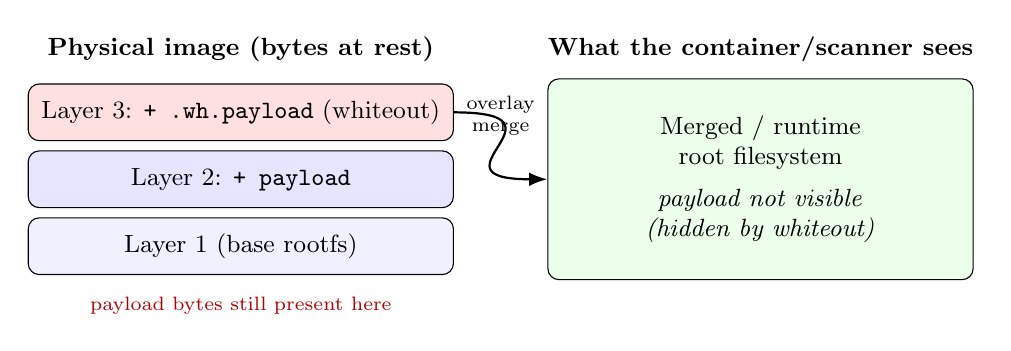
\begin{tikzpicture}[
  layer/.style={draw, rounded corners, minimum width=5.4cm, minimum height=0.72cm,
                align=center, font=\small},
  file/.style={font=\small\ttfamily},
]
% physical layers
\node[layer, fill=blue!6]  (l1) at (0,0)   {Layer 1 (base rootfs)};
\node[layer, fill=blue!10] (l2) at (0,0.85){Layer 2: \texttt{+ payload}};
\node[layer, fill=red!12]  (l3) at (0,1.7) {Layer 3: \texttt{+ .wh.payload} (whiteout)};

\node[font=\small\bfseries] at (0,2.5) {Physical image (bytes at rest)};

% merged view
\begin{scope}[xshift=6.6cm]
\node[layer, fill=green!8, minimum height=2.55cm] (mv) at (0,0.85)
   {Merged / runtime\\ root filesystem\\[4pt]
    \textit{payload not visible}\\ \textit{(hidden by whiteout)}};
\node[font=\small\bfseries] at (0,2.5) {What the container/scanner sees};
\end{scope}

\draw[-{Latex}, thick] (l3.east) .. controls +(1.6,0) and +(-1.6,0) .. (mv.west)
  node[midway, above, font=\scriptsize, align=center] {overlay\\ merge};

\node[font=\scriptsize, align=center, red!70!black] at (0,-0.75)
  {payload bytes still present here};
\end{tikzpicture}
\caption{Whiteout smuggling. The payload is added in layer~2 and ``deleted'' in
layer~3. It disappears from the merged runtime filesystem but persists in the
layer-2 blob, invisible to rootfs-only scanners.}
\label{fig:whiteout}
\end{figure*}

\subsection{Steganographic carriers in images}
We consider two carrier families that exploit different properties:
\begin{description}
\item[Structural carrier (whiteout).] The payload is a real file added low and
whited-out high. It is invisible in the merged filesystem but leaves a
\emph{structural} trace across layers: an add followed by a delete of the same
path.
\item[Content-embedded carrier (appended data).] The payload is hidden inside a
benign asset that \emph{remains present} in the root filesystem---here, appended
after the \texttt{IEND} chunk of a valid PNG. The image still renders; there is
no whiteout and no misplaced executable. At rest it is essentially indistinguishable
from a legitimate asset.
\end{description}
These carriers are complementary from the defender's viewpoint, which motivates a
two-layer approach.

\subsection{eBPF}
eBPF lets small, verified programs run in the Linux kernel and attach to events
such as system-call entry/exit. Because it observes at the kernel boundary, eBPF
is unaffected by user-space or union-filesystem abstractions: it sees the actual
\texttt{open}, \texttt{read}, \texttt{memfd\_create}, and \texttt{execveat}
operations a process performs, regardless of how the container presents its
filesystem. This vantage point is what lets us detect the \emph{use} of a hidden
payload even when its presence is concealed.

%======================================================================
\section{Threat Model}
%======================================================================
We assume an adversary who can influence the contents of a distributed image
(e.g., a compromised build step, a malicious base image, or an insider) and whose
goal is to ship a payload past image-scanning defenses and use it at runtime. The
defender can (a) statically scan images before deployment and (b) run a runtime
sensor on hosts. We do \emph{not} assume the adversary has escaped the container
or obtained host privileges; the content-embedded carrier is decoded by a normal
in-container process from an asset the container legitimately contains. Denial of
service, covert network channels, and hardware side channels are out of scope.

%======================================================================
\section{Design of the Dataset and Experiment}
\label{sec:design}
%======================================================================
To attribute any detection difference to the hiding technique alone, we hold the
payload bytes constant and vary only delivery.

\paragraph{Payload.} A tiny, freestanding (no libc) x86-64 ELF of about one
kilobyte whose entire effect is to create the marker file
\texttt{/tmp/stego\_marker} and print one line. The same bytes are used in every
variant. A freestanding ELF is used rather than a shell script because a shebang
script cannot be executed filelessly from an anonymous memory file
(Section~\ref{sec:dynamic}).

\paragraph{Image triplet.} Table~\ref{tab:triplet} lists the three variants built
on the same base web-server image.

\begin{table}[t]
\caption{The clean/plain/stego image triplet. Payload bytes are identical;
only delivery differs.}
\label{tab:triplet}
\small
\begin{tabular}{@{}lll@{}}
\toprule
Variant & Delivery & Expected difficulty \\
\midrule
Clean & none (control) & --- \\
Plain & payload as an ordinary file & easy (visible) \\
Stego & payload hidden (whiteout / appended-data) & hard (concealed) \\
\bottomrule
\end{tabular}
\end{table}

\paragraph{Control ladder for the runtime experiment.} Because ``run a payload
from memory'' is itself a generic evasion technique, we add an intermediate
variant so that the runtime detector's power can be attributed specifically to
\emph{extraction} and not merely to fileless execution
(Table~\ref{tab:ladder}).

\begin{table}[t]
\caption{Runtime control ladder. Same payload bytes throughout; each step adds
one behavior. B1 isolates generic fileless execution from stego extraction.}
\label{tab:ladder}
\small
\begin{tabular}{@{}llccc@{}}
\toprule
 & Mechanism & Carrier read & Decode & Fileless exec \\
\midrule
B0 & normal \texttt{execve} & --- & --- & --- \\
B1 & \texttt{memfd}+\texttt{execveat} & payload file & --- & \checkmark \\
C  & extract + run & carrier asset & \checkmark & \checkmark \\
\bottomrule
\end{tabular}
\end{table}

%======================================================================
\section{Static Detection Layer}
\label{sec:static}
%======================================================================
The static detector consumes an image (as a docker-archive tarball or an OCI
layout) and iterates each layer archive \emph{in application order}, maintaining a
map of every file introduced together with metadata (executable bit, size, byte
entropy). It emits findings at three severities. The key departures from a naive
scanner are that it (i) never matches on payload filenames and (ii) treats
whiteouts as evidence rather than noise.

\paragraph{Add-then-hide correlation.} When the detector encounters a whiteout
for path $p$, it checks whether $p$ was previously \emph{added as an executable}
in a lower layer. If so, this is the structural fingerprint of whiteout
smuggling---an executable that is present in the physical image yet absent from
the merged filesystem---and is reported as high severity. Opaque whiteouts and
ordinary deletions (no matching executable add) are downgraded.

\paragraph{Misplaced executables and entropy.} Independently, an executable
introduced into a data-only directory (e.g., \texttt{/var/log}, \texttt{/tmp})
is flagged regardless of its name, capturing the plain-delivery case without a
signature; a high-entropy executable is flagged as possibly packed. These
heuristics are corpus-tuned and would require an allowlist for production base
images.

\paragraph{Baseline.} We retain a deliberately naive scanner---signature-only,
whiteout-blind, docker-archive-only---as the comparison baseline. It represents
the rootfs/signature scanners common today and is expected to miss both concealed
and renamed payloads.

%======================================================================
\section{Dynamic Detection Layer}
\label{sec:dynamic}
%======================================================================
The dynamic layer targets the \emph{content-embedded} carrier, which the static
layer cannot see at rest. The attacker's runtime behavior forms a distinctive
chain:
\[
\begin{aligned}
&\texttt{openat(asset)} \to \texttt{read} \to \text{[decode]} \to\\
&\texttt{memfd\_create} \to \texttt{write} \to \texttt{execveat}.
\end{aligned}
\]
The process opens a benign asset, reads it, decodes the hidden region, writes the
result into an anonymous in-memory file (\texttt{memfd}), and executes it directly
with \texttt{execveat} and \texttt{AT\_EMPTY\_PATH}---i.e., \emph{filelessly},
leaving no on-disk artifact.

\paragraph{Separating extraction from fileless execution.} Fileless execution
alone is a known, generic technique that runtime tools already surface. To
identify \emph{steganographic} behavior specifically, we observe that an extractor
\emph{reads much more than it executes}: it consumes a whole carrier asset but
runs only the small decoded region. We therefore compute, per process, the ratio
of bytes read to bytes written into the executed \texttt{memfd}. A ratio near
$1{:}1$ indicates plain fileless execution (variant B1); a large ratio indicates
extraction from a carrier (variant C). The detector (an eBPF/\texttt{bpftrace}
program) is entirely filename-agnostic: it keys on the memfd-to-\texttt{execveat}
relationship and on this byte ratio, never on payload names.

\paragraph{Provenance caveat.} The byte ratio is a per-process \emph{sum}, a proxy
for provenance rather than true data-flow taint. It establishes ``a fileless
execution preceded by disproportionately large reads,'' not ``these exact bytes
came from that file.'' Full taint tracking is future work
(Section~\ref{sec:limitations}).

%======================================================================
\section{Evaluation}
\label{sec:eval}
%======================================================================
We report results for the two carriers. Static results are verdicts of the two
scanners over the image triplet and, for generalization, over six base images
spanning databases and language runtimes; dynamic results are byte-ratio
measurements captured live from the eBPF detector as each control-ladder variant
executes.

\subsection{Static verdicts}
Table~\ref{tab:static} contrasts the naive baseline with the layer-aware
detector. The baseline misses the concealed payload and, because the plain
payload is not named like its signature, misses that too---illustrating signature
brittleness. The layer-aware detector flags the plain case (misplaced executable)
and the whiteout case (add-then-hide), while leaving the clean image untouched.

\begin{table}[t]
\caption{Static detection over the image triplet. ``miss'' for the baseline on
Plain reflects a payload name outside its signature set.}
\label{tab:static}
\small
\begin{tabular}{@{}lcc@{}}
\toprule
Image & Naive baseline & Layer-aware (ours) \\
\midrule
Clean & clean & clean \\
Plain & \textbf{miss} & \textbf{detect} (misplaced exec) \\
Stego (whiteout) & \textbf{miss} & \textbf{detect} (add-then-hide) \\
\bottomrule
\end{tabular}
\end{table}

\paragraph{Generalization across base images.}
To check that detection is not specific to a single base, we repeated the
clean/plain/stego construction on six widely used images spanning databases and
language runtimes over three distributions (Table~\ref{tab:general}). The
layer-aware detector flagged all $12$ malicious variants ($6$ plain via misplaced
executable, $6$ stego additionally via add-then-hide) and raised \emph{zero}
findings on the six clean bases. Detection therefore transfers across base
images, and the location/entropy heuristics did not misfire on real database and
runtime images.

\begin{table}[t]
\caption{Generalization of the layer-aware static detector. Plain and Stego are
malicious (want detection); Clean is a false-positive check (want none). All
verdicts as desired.}
\label{tab:general}
\small
\begin{tabular}{@{}llccc@{}}
\toprule
Base image & Class / distro & Clean & Plain & Stego \\
\midrule
\texttt{postgres:latest}   & db / debian      & clean & \checkmark & \checkmark \\
\texttt{redis:alpine}      & db / alpine      & clean & \checkmark & \checkmark \\
\texttt{mariadb:latest}    & db / ubuntu      & clean & \checkmark & \checkmark \\
\texttt{python:3.12-slim}  & runtime / debian & clean & \checkmark & \checkmark \\
\texttt{node:20-alpine}    & runtime / alpine & clean & \checkmark & \checkmark \\
\texttt{golang:1.22-alpine}& runtime / alpine & clean & \checkmark & \checkmark \\
\bottomrule
\end{tabular}
\end{table}

\subsection{Dynamic byte ratio}
We measured the ratio live with the eBPF detector attached to the host kernel
(run in a privileged container so it observes the host's syscalls), detonating
each control-ladder variant in turn. B0 (normal \texttt{execve}) produced no
event, correctly ignored as it uses no anonymous memory file. B1 read
1904\,B (its 1072\,B payload plus loader header reads) and executed 1072\,B, a
$1{:}1$ ratio flagged as plain fileless execution. C read 18497\,B (the carrier
asset) but executed only the 1072\,B decoded payload, a $17{:}1$ ratio---well
above the alerting threshold and cleanly separated from B1
(Figure~\ref{fig:ratio}). The detector
keys only on the memfd-to-\texttt{execveat} relation and this ratio; it never
inspects payload names.

\begin{figure}[t]
\centering
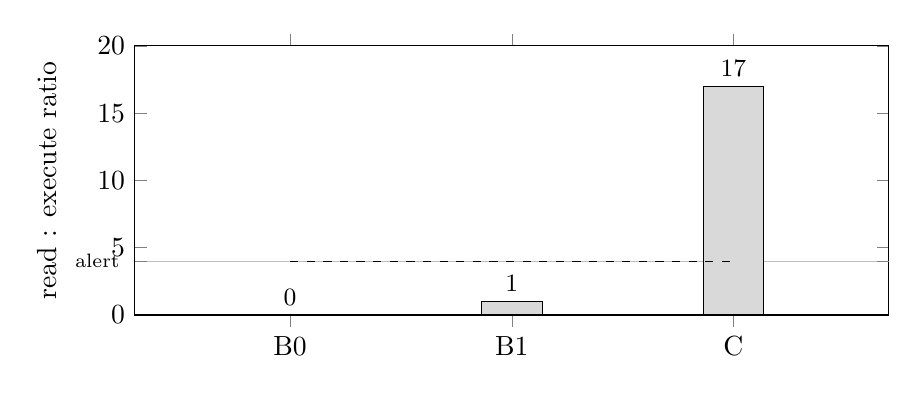
\begin{tikzpicture}
\begin{axis}[
  width=0.92\linewidth, height=5cm,
  ybar, bar width=22pt,
  ymin=0, ymax=20,
  ylabel={read : execute ratio},
  symbolic x coords={B0, B1, C},
  xtick=data,
  nodes near coords,
  nodes near coords style={font=\small},
  enlarge x limits=0.35,
  extra y ticks={4}, extra y tick labels={\scriptsize alert},
  extra y tick style={grid=major, tick label style={xshift=-2pt}},
]
\addplot[fill=gray!30] coordinates {(B0,0) (B1,1) (C,17)};
\draw[dashed] (axis cs:B0,4) -- (axis cs:C,4);
\end{axis}
\end{tikzpicture}
\caption{Read-to-execute byte ratio per control-ladder variant, measured live via
eBPF. B0 does no fileless execution (shown as~0). B1 (plain fileless) sits at
$1{:}1$; C (stego extraction) at $17{:}1$. The dashed line is the alert threshold.}
\label{fig:ratio}
\end{figure}

\subsection{Coverage crossover}
The central claim is complementarity, and it holds at both carriers we
measured. For the \emph{structural} (whiteout) carrier, the static detector fires
(add-then-hide; Tables~\ref{tab:static},~\ref{tab:general}) while nothing is
extracted at container runtime, so the dynamic layer does not apply. For the
\emph{content-embedded} (appended-data) carrier, the static detector reports the
image clean---the carrier is a valid asset in a normal path and the extractor is
an ordinary binary, leaving no structural trace---while the dynamic detector
fires on the extraction (Figure~\ref{fig:ratio}). Neither layer covers both
carriers alone; their union does (Figure~\ref{fig:crossover}). This is a measured
two-point result, not an interpolated curve: each cell corresponds to an actual
scan or trace.

\begin{figure}[t]
\centering
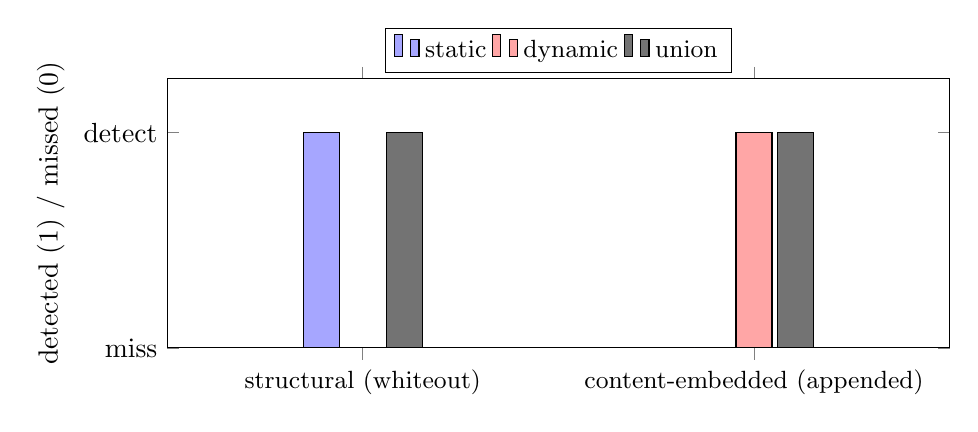
\begin{tikzpicture}
\begin{axis}[
  width=0.95\linewidth, height=5cm,
  ybar, bar width=13pt,
  ymin=0, ymax=1.25,
  ylabel={detected (1) / missed (0)},
  symbolic x coords={structural (whiteout), content-embedded (appended)},
  xtick=data,
  x tick label style={font=\small, align=center},
  ytick={0,1}, yticklabels={miss, detect},
  enlarge x limits=0.5,
  legend style={font=\small, at={(0.5,1.02)}, anchor=south, legend columns=3},
]
\addplot[fill=blue!35]  coordinates {(structural (whiteout),1) (content-embedded (appended),0)};
\addplot[fill=red!35]   coordinates {(structural (whiteout),0) (content-embedded (appended),1)};
\addplot[fill=black!55] coordinates {(structural (whiteout),1) (content-embedded (appended),1)};
\legend{static, dynamic, union}
\end{axis}
\end{tikzpicture}
\caption{Measured coverage at the two carriers. The static (layer-aware) detector
catches the structural carrier but misses the content-embedded one; the dynamic
(eBPF) detector does the reverse; their union catches both. Each bar is a real
scan or live trace, not an interpolation.}
\label{fig:crossover}
\end{figure}

%======================================================================
\section{Related Work}
%======================================================================
Malicious-image and supply-chain scanners inspect image contents for known-bad
files, secrets, and vulnerable packages, typically over the merged filesystem or
per-layer file listings; they are effective against visible artifacts but, as our
baseline illustrates, are weak against concealment that leaves no signature.
Runtime security tools such as Falco and Tetragon detect suspicious syscall and
process behavior generically---including fileless execution---but do not, to our
knowledge, distinguish steganographic \emph{extraction} from other fileless
activity, which is precisely the gap our byte-ratio signal targets. Classical
steganalysis focuses on statistical detection within a single medium; our
contribution is to place detection at the two structural seams that containers
introduce---image layers and the runtime syscall boundary---rather than within a
single file. A full quantitative comparison against Falco and Tetragon on the same
samples is planned for the extended version.

%======================================================================
\section{Limitations}
\label{sec:limitations}
%======================================================================
These results are preliminary: one carrier per family and a benign payload. The
static heuristics (data-directory location lists, entropy threshold) are tuned to
the corpus; although they produced no false positives on the six clean base images
we tested (Section~\ref{sec:eval}), a production deployment over a large image
population would still require allowlisting to bound the false-positive rate. The
dynamic byte-ratio signal is a provenance proxy, not data-flow taint, and can in
principle be evaded by laundering the carrier read and the execution across
separate processes; per-process correlation would then need to become
cross-process lineage tracking. We demonstrate the eBPF detector firing live on
the control ladder, but a large-scale evaluation of its false-positive rate on
representative production workloads (e.g., runtimes that legitimately use
anonymous memory files) remains future work. Finally, we study appended-data and
whiteout carriers; padding, gzip-metadata, and file-ordering carriers remain to be
evaluated.

%======================================================================
\section{Conclusion}
%======================================================================
Container images give adversaries two very different places to hide a payload: in
the physical bytes of a lower layer that the runtime pretends to have deleted, and
inside a benign asset that is decoded only when it runs. We showed that a single
vantage point cannot cover both, and that a static layer-aware scanner and a
dynamic eBPF sensor are complementary---the former catching structural
add-then-hide smuggling, the latter catching runtime extraction by its
read-to-execute byte ratio, both without relying on payload names. The union of
the two closes the coverage gap on our controlled dataset. We release the dataset,
detectors, and control ladder to serve as an early, reproducible baseline for
detecting hidden channels in OCI images.

\paragraph{Availability.} All code and the image-building scripts are available in
the accompanying repository.

%\bibliographystyle{ACM-Reference-Format}
%\bibliography{refs}
\begin{thebibliography}{9}
\small
\bibitem{ociimage} The Open Container Initiative. \emph{OCI Image Format
Specification}. \url{https://github.com/opencontainers/image-spec}.
\bibitem{overlayfs} The Linux Kernel. \emph{Overlay Filesystem Documentation}.
\url{https://www.kernel.org/doc/html/latest/filesystems/overlayfs.html}.
\bibitem{ebpf} B.~Gregg. \emph{BPF Performance Tools}. Addison-Wesley, 2019.
\bibitem{falco} The Falco Project (CNCF). \url{https://falco.org}.
\bibitem{tetragon} Cilium/Isovalent. \emph{Tetragon}.
\url{https://github.com/cilium/tetragon}.
\bibitem{provos} N.~Provos and P.~Honeyman. Hide and Seek: An Introduction to
Steganography. \emph{IEEE Security \& Privacy}, 2003.
\end{thebibliography}

\end{document}
